\documentclass{beamer}
\usepackage[brazilian]{babel}
\usepackage[utf8]{inputenc}
\usepackage[T1]{fontenc}
\usepackage{minted}
\usepackage{algorithmic}
\usepackage[brazilian]{algorithm}
\usepackage{amsthm}
\usepackage{graphicx}
\usemintedstyle{tango}

\renewcommand{\algorithmicrequire}{\textbf{Entrada:}}
\renewcommand{\algorithmicensure}{\textbf{Saída:}}
\renewcommand{\algorithmicend}{\textbf{fim}}
\renewcommand{\algorithmicif}{\textbf{se}}
\renewcommand{\algorithmicthen}{\textbf{então}}
\renewcommand{\algorithmicelse}{\textbf{else}}
\renewcommand{\algorithmicelsif}{\algorithmicelse\ \algorithmicif}
\renewcommand{\algorithmicendif}{\algorithmicend\ \algorithmicif}
\renewcommand{\algorithmicfor}{\textbf{para}}
\renewcommand{\algorithmicforall}{\textbf{para todos}}
\renewcommand{\algorithmicdo}{\textbf{faça}}
\renewcommand{\algorithmicendfor}{\algorithmicend}
\renewcommand{\algorithmicwhile}{\textbf{enquanto}}
\renewcommand{\algorithmicendwhile}{\algorithmicend}
\renewcommand{\algorithmicloop}{\textbf{loop}}
\renewcommand{\algorithmicendloop}{\algorithmicend\ \algorithmicloop}
\renewcommand{\algorithmicrepeat}{\textbf{repita}}
\renewcommand{\algorithmicuntil}{\textbf{enquanto}}
\renewcommand{\algorithmicprint}{\textbf{imprima}}
\renewcommand{\algorithmicreturn}{\textbf{retorne}}
\renewcommand{\algorithmictrue}{\textbf{verdadeiro}}
\renewcommand{\algorithmicfalse}{\textbf{falso}}


\renewcommand{\theFancyVerbLine}{
  \sffamily\textcolor[rgb]{0.5,0.5,0.5}{\scriptsize\arabic{FancyVerbLine}}}

\AtBeginSection{\frame{\sectionpage}}
\newtranslation[to=brazilian]{Section}{Se\c c\~ao}

\newtheorem{mydef}{Defini\c c\~ao}

\title{\emph{There and back again}\\Convertendo aut\^omatos para gram\'aticas}
\author{Lucas Virgili}
\date{}

\begin{document}

\begin{frame}[fragile]
  \titlepage
\end{frame}

\begin{frame}[fragile]
  \frametitle{\emph{The map}}
  \begin{center}
  \includegraphics[width=0.9\textwidth]{estruturabranco.png}
  \end{center}
\end{frame}

\begin{frame}[fragile]
  \frametitle{De matriz para regex}
  \begin{itemize}
  \item Implementei o m\'etodo idiota, doravante chamado de m\'etodo
    chamado de m\'etodo L. (de Lucas)
    \begin{itemize}
    \item Basicamente uma ``reinterpreta\c c\~ao'' do algoritmo de
      Floyd-Warshall
    \end{itemize}
  \item Comecei a implementar o algoritmo de \emph{state removal}
  \item Enquanto eu procurava por heur\'isticas para qual estado
    remover primeiro, encontrei um m\'odulo de python chamado FAdo
  \item J\'a tinha implementado as heur\'isticas!
  \end{itemize}
\end{frame}

\begin{frame}[fragile]
  \frametitle{Comparando os m\'etodos}
  \begin{itemize}
  \item Usando os m\'etodos implementados no FAdo e o m\'etodo L em
    aut\^omatos finitos aleat\'orios, eu analisei qual o m\'etodo
    gerava a menor regex.
  \item Os testes n\~ao puderam ser feitos com aut\^omatos muito
    grandes (muitos estados) nem com um alfabeto muito extenso, j\'a
    que meu computador \'e uma droga e os algoritmos tem complexidades
    que deixam a desejar.
  \end{itemize}
\end{frame}

\begin{frame}[fragile]
  \frametitle{0 e 1!}
  \begin{itemize}
  \item $\Sigma = \{0, 1\}$ e 2 estados.
  \end{itemize}
  \begin{center}
  \includegraphics[width=0.9\textwidth]{plot2_2.png}
  \end{center}
\end{frame}

\begin{frame}[fragile]
  \frametitle{$|\Sigma| = 5$ e 6 estados}
  \begin{center}
  \includegraphics[width=0.9\textwidth]{plot5_6.png}
  \end{center}
\end{frame}

\begin{frame}[fragile]
  \frametitle{$|\Sigma| = 10$ e 7 estados}
  \begin{center}
  \includegraphics[width=0.9\textwidth]{plot10_7.png}
  \end{center}
\end{frame}

\begin{frame}[fragile]
  \frametitle{O veredicto}
  \begin{itemize}
  \item Usar elimina\c c\~ao de estados \'e r\'apido e gera
    express\~oes de tamanhos semelhantes aos outros m\'etodos.
  \end{itemize}
\end{frame}

\begin{frame}[fragile]
  \frametitle{De regex \`a gram\'atica}
  \begin{itemize}
  \item Dada a regex, \'e simples obter uma gram\'atica equivalente:
    basta nomear cada n\~ao terminal e, para cada um deles, formalizar
    as uni\~oes e os fechos.
  \end{itemize}
\end{frame}

\begin{frame}[fragile]
  \frametitle{A cobaia}
  \begin{center}
    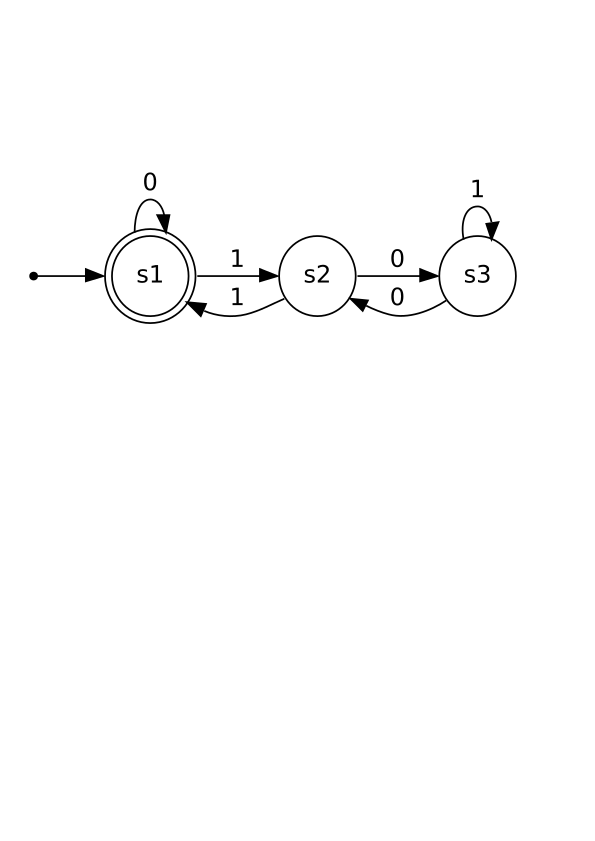
\includegraphics[width=0.8\textwidth]{output.png}
  \end{center}
\end{frame}

\begin{frame}[fragile]
  \frametitle{A cobaia virou uma regex...}
  \begin{itemize}
  \item Sua regex:\\
    ((0 + (1 1)) + (((1 0) (1 + (0 0))*) (0 1)))*
  \end{itemize}
\end{frame}

\begin{frame}[fragile]
  \frametitle{E a regex virou uma gram\'atica!}
  \begin{itemize}
  \item A = \{0\}
  \item B = (1 1)
  \item C = (A B)
  \item D = \{C\}
  \item E = (1 0)
  \item F = \{1\}
  \item G = (0 0)
  \item H = (F G)
  \item I = [H]
  \item J = (E I)
  \item K = (0 1)
  \item L = (J K)
  \item M = (D L)
  \item N = [M]
  \end{itemize}
\end{frame}

\end{document}